
%%
%% CIS121 Fall 2015 in a Nutshell
%% @author jtcho - jonathan.t.cho@gmail.com
%%
%% Must be compiled using XeLaTeX.
%% xelatex --shell-escape %file
%%
%% TODO: Shellsort!
%%
%% Have any questions/found a bug? Shoot me an email!

\documentclass[12pt, fleqn]{general}

\usepackage{multicol}

\newlength\tindent
\setlength{\tindent}{\parindent}
\setlength{\parindent}{0pt}
\renewcommand{\indent}{\hspace*{\tindent}}
\setlength{\mathindent}{0pt}

\begin{document}

\titleformat{\section}{\normalfont\LARGE\bfseries\centering}{\thesection}{1em}{}[{\titlerule[0.6pt]}]

\section*{CIS121 in a ``Nutshell" (Fall 2015)}
\vspace{-20pt}

%\begingroup
    \fontsize{10pt}{12pt}
%\endgroup
\begin{multicols*}{2}
[{\small \begin{center}Comprehensive guide to all things CIS121. The information here is probably much more than you need to know for the exam. Extra sections that won't be tested are marked with asterisks.\end{center}}]

    %%%%%%%%%%%%%%%%%%%%
    %% TILDE NOTATION %%
    %%%%%%%%%%%%%%%%%%%%
    {\large \underline{Tilde Notation}}\\

    $f(n) \sim g(n)$ \emph{if and only if} $\lim_{n\rightarrow\infty} \frac{f(n)}{g(n)} = 1$\\ 

    $\therefore$ $f$ and $g$ must be \emph{asymptotically equal}. Represents both an upper and lower bound, does \textbf{not} ignore constant multipliers (e.g. $n \sim n + 1$ but $n \not\sim 3n + 1$) Comparable to Big-$\Theta$ when lower and upper bound constants are $1$.\\

    %%%%%%%%%%%%%%%%%%%%%%%%%%%%%%
    %% BACCHMAN-LANDAU NOTATION %%
    %%%%%%%%%%%%%%%%%%%%%%%%%%%%%%
    {\large \underline{Bacchman-Landau Notation}}\\

    $f(n) \in O(g(n))$ if $\exists\; c,n_0$ s.t. $f(n) \leq c g(n)\; \forall\; n \geq n_0$\\
    $\therefore$ $g$ multiplied by some positive constant is an upper bound for $f$.\\

    $f(n) \in \Omega(g(n))$ if $\exists\; c,n_0$ s.t. $f(n) \geq c g(n)\;\forall\; n \geq n_0$\\
    $\therefore$ $g$ multiplied by some positive constant is a lower bound for $f$.\\

    $f(n) \in \Theta(g(n))$ if $\exists\; c_1, c_2, n_0$ s.t. $f(n) \leq c_1 g(n)$ and $f(n) \geq c_2 g(n)\;\forall\; n \geq n_0$\\
    $\therefore$ $f(n) \in O(g(n))$ and $f(n) \in \Omega(g(n))$. $g$ is an asymptotically tight bound for $f$.\\

    $f(n) \in o(g(n))$ if $\forall c > 0\; \exists\; n_0 > 0$ s.t. $f(n) < c g(n)\; \forall\; n \geq n_0$. \vspace{-5pt}
    \begin{align*}
        f(n) \in o(g(n)) &\implies \lim_{n\rightarrow\infty} \frac{f(n)}{g(n)} = 0\\
                         &\implies f(n) \in O(g(n))
    \end{align*}
    $\therefore$ $g$ is a strict upper bound for $f$\\

    $f(n) \in \omega(g(n))$ if $\forall c > 0\; \exists\; n_0 > 0$ s.t. $f(n) > c g(n)\; \forall\; n \geq n_0$.\vspace{-5pt}
    \begin{align*}
        f(n) \in \omega(g(n)) &\implies \lim_{n\rightarrow\infty} \frac{f(n)}{g(n)} = \infty\\
                            &\implies f(n) \in \Omega(g(n))
    \end{align*}
    $\therefore$ $g$ is a strict lower bound for $f$.\\

    %%%%%%%%%%%%%%%%%%%
    %% CASE ANALYSIS %%
    %%%%%%%%%%%%%%%%%%%

    {\large \underline{Best, Worst, Average Case Analysis}}\\

    \textbf{best case analysis}: examining the optimal runtime/space usage of an algorithm. Not often useful.\\

    \textbf{worst case analysis}: examining the worst case runtime/space usage of an algorithm. Often of interest because it is important to know how much time or space is needed to guarantee an algorithm's success.\\

    \textbf{average case analysis}: analysis of the runtime/space usage of an algorithm for an \emph{average} input. \textbf{NOT AMORTIZED ANALYSIS.} \underline{Note}: What constitutes an average input may not always be clear - so an algorithm may not admit an average case analysis. Involves use of probabilistic analysis to determine expected running times/space usage.\\

    %%%%%%%%%%%%%%%%%%%%%%%%%
    %% METHOD OF ITERATION %%
    %%%%%%%%%%%%%%%%%%%%%%%%%
    {\large \underline{Method of Iteration for Recurrences*}}\\

    Let $T(n) = a T(n/b) + f(n)$. Given base case $T(u) = c$ where $u = n/b^k$, $T(n)$ can be solved by simplifying $T(n) = f(n) + a f(\frac{n}{b}) + a^2 f(\frac{n}{b^2}) + \cdots + a^k f(\frac{n}{b^k}) + c\cdot a^{k+1}$.\\

    %%%%%%%%%%%%%%%%%%%%%%%%%%%
    %% GEOMETRIC SUM FORMULA %%
    %%%%%%%%%%%%%%%%%%%%%%%%%%%
    {\large \underline{Geometric Sum Formula}}
    \begin{align*}
        \sum_{i = 0}^k q^i = \frac{q^{k+1} - 1}{q - 1} = \frac{1-q^{k+1}}{1-q}
    \end{align*}

    %%%%%%%%%%%%%%%%%%%%%%
    %% L'HOPITAL'S RULE %%
    %%%%%%%%%%%%%%%%%%%%%%
    {\large \underline{L'Hopital's Rule}}\\

    Consider functions $f$ and $g$ that are differentiable except possibly at point $c$, such that $\lim_{n\rightarrow c} f(n) = \lim_{n\rightarrow c} g(n) = 0 \text{ or } \pm \infty$. If the limit $\lim_{n\rightarrow c}\frac{f'(n)}{g'(n)}$ exists and $g'(n) \neq 0\;\forall\; n \neq c$,
    $$
        \lim_{n\rightarrow c} \frac{f(n)}{g(n)} = \lim_{n\rightarrow c} \frac{f'(n)}{g'(n)}
    $$
    
\end{multicols*}
    
    %%%%%%%%%%%%%%%%%%%%%%%%
    %% COMMON RECURRENCES %%
    %%%%%%%%%%%%%%%%%%%%%%%%

    {\large \underline{Common Recurrences}}

    \begin{center}
    \begin{tabular}{|c|c|c|}\hline
    \textbf{Recurrence}&\textbf{Solution}&\textbf{Algorithm}\\\hline
    $T(n) = \begin{cases} T(n-1) + n & n \geq 1\\ 0 & \text{ otherwise }\end{cases}$& $T(n) = {n+1 \choose 2} = \frac{1}{2}n(n+1)$&Selection Sort\\\hline
    $T(n) = \begin{cases} T(n/2) + c & n \geq 2\\ 1 & \text{ otherwise }\end{cases}$& $T(n) = c \log n + 1$ & Binary Search\\\hline
    $T(n) = \begin{cases} T(n/2) + n & n \geq 2\\ 1 & \text{ otherwise }\end{cases}$& $T(n) = 2n - 1$ & Selection Problem\\\hline
    $T(n) = \begin{cases}2 T(n/2) + n & n \geq 2\\ 1 & \text{otherwise}\end{cases}$& $T(n) = n \log n + n$ & Mergesort\\\hline
    \end{tabular}\\
    \end{center}

\begin{multicols*}{2}

    %%%%%%%%%%%%%%%%%%%
    %% STACKS/QUEUES %%
    %%%%%%%%%%%%%%%%%%%
    {\large \underline{Stacks/Queues}}\\

    Stacks (\textbf{LIFO/FILO}): The last element to be inserted is the first one to be removed. Imagine a box where only one end is open; to get to the stuff at the bottom, you have to take out all the stuff on top first.\\

    Queues (\textbf{FIFO}): The first element to be inserted is the first one to be removed. Imagine a box where both ends are open. Whatever you put into the box will fall through the other end first.\\

    Can be implemented using a linked list or a resizing array. A \texttt{Deque} is an ADT that functions as both a \texttt{Stack} and a \texttt{Queue}.\\

    \texttt{PUSH}, \texttt{POP}, \texttt{PEEK} in worst-case $O(1)$ for the linked list. \texttt{PUSH} and \texttt{POP} in amortized $O(1)$ for the resizing array, \texttt{PEEK} in worst-case $O(1)$. (Same for the \texttt{Queue}'s head/tail methods.)\\

    %%%%%%%%%%%%%%%%%%%%%%%%
    %% AMORTIZED ANALYSIS %%
    %%%%%%%%%%%%%%%%%%%%%%%%

    {\large \underline{Amortized Analysis}}\\

    Used to examine the average cost of an operation over a sequence of such operations. If an operation is cheap most of the time and expensive in some, we can average out the cost of the expensive calls. (e.g. resizing array)\\

    %%%%%%%%%%%%%%%%
    %% UNION FIND %%
    %%%%%%%%%%%%%%%%
    \vspace{-20pt}{\large \underline{Union Find}}

    Data structure that maintains a set of elements partitioned into disjoint subsets.

    •\texttt{FIND(x)} - returns the representative element of the subset $x$ is in\\
    •\texttt{UNION(x,y)} - unions the two disjoint sets that $x, y$ are in

    Implemented as a \emph{disjoint forest}, where the representative element of each set is the root of each tree. The representative elements can be used to identify whether two elements are in the same partition.

    \textbf{Optimizations}:\\
    • \emph{Union by Rank} - when union-ing two trees, attach root of smaller one to root of larger one
    • \emph{Path Compression} - flattens tree structure in \texttt{FIND} by setting each visited node's parent to the root

    Together, the above optimizations give amortized $O(\alpha(n))$ for \texttt{FIND} and \texttt{UNION}, where $\alpha(n)$ is the inverse Ackermann function (which grows SUPER DUPER slowly).

    \textbf{Applications}:\\
    •Are vertices $u$ and $v$ in the same connected component in an undirected graph $G$?\\
    •Would adding an edge between vertices $u$ and $v$ create a cycle in a undirected graph $G$?\\
    •Kruskal's Algorithm for Computing a MST

    \newpage

    %%%%%%%%%%%%%%%%%%%%%%
    %% ELEMENTARY SORTS %%
    %%%%%%%%%%%%%%%%%%%%%%
    {\large \underline{Elementary Sorts}}\\

    \emph{stable sort} - a sorting algorithm that preserves the relative order of elements with equal values (e.g. \texttt{sort([f, e, a, d, a', g])} results in \texttt{[a, a', d, e, f, g]}, preserving the relative order of the \texttt{a} keys)\\

    \emph{in-place sort} - a sorting algorithm that only uses $O(1)$ additional memory\\

    \emph{online sort} - a sorting algorithm that can sort a list as it receives it as compared to needing the full input all at once. (e.g. selection sort, an offline sort, requires the minimum of the entire \emph{unsorted} array at each iteration. On the other hand, insertion sort, an online sort, inserts an element from the unsorted array in its proper position in the sorted array at each iteration, independent of future elements.)\\

    \emph{adaptive sort} - a sorting algorithm that is more efficient if the input is already (at least) partially ordered\\

    \textbf{Selection Sort}\\

    Builds sorted list one element at a time with each iteration. Inefficient for large lists, tends to perform worse than insertion sort. In-place, offline, \emph{can} be stable depending on implementation.\\

    \underline{Algorithm.} Grows sorted sublist $L$ from left (initially empty). Pick smallest element from unsorted sublist $R$ and swap with the leftmost element in the unsorted sublist. Grow $L$ by 1 index and shrink $R$ by 1 index. Repeat until $R$ is empty.\\

    \underline{Runtime.} At each iteration we search $R$ for the smallest element. $R$ starts as size $n$ and shrinks by $1$ per loop: $$n + (n-1) + (n-2) + ... + 1 = \frac{1}{2} n(n+1) = \Theta(n^2)$$

    \textbf{Insertion Sort}\\

    \begin{figure*}[t]
        \centering
        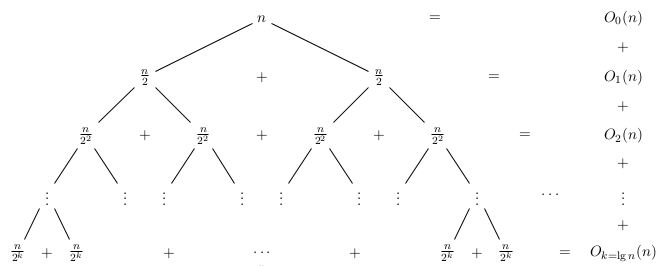
\includegraphics[width=\textwidth*7/8]{mergesort.png}
        \caption*{\emph{Recursion tree for Mergesort. Total work done at each level is $O(n)$.}}
    \end{figure*}

    Builds sorted list one element at a time with each iteration. Inefficient for large lists, but simple, efficient for small lists, adaptive, stable, in-place, online.\\

    \underline{Algorithm.} Grows sorted sublist $L$ from left (initially empty). Pick first element $x$ from unsorted sublist $R$. Compare $x$ with the element to its left. If strictly smaller, swap the two values and repeat until at $x$ is at index $i$ s.t. $A[i-1] \leq x < A[i+1]$. Grow $L$ by 1 and shrink $R$ by 1. Repeat until $R$ is empty.\\

    \underline{Runtime.} \emph{Worst-case input} is a completely reversed list. Will require $1 + 2 + ... + (n-1) = {n \choose 2} = \Theta(n^2)$ comparisons. (e.g. on the last iteration, the last element in $R$ is the smallest element and will have to be swapped down with the other $n-1$ elements in $L$).\\
    
    \emph{Average-case analysis:} Define indicator variable $$I_{i,j} = \begin{cases} 1 & \text{if $(i,j)$ is an inversion}\\ 0 &\text{if not}\end{cases}$$ Let $I = \sum_{i < j} I_{i,j}$. Observe that swapping an adjacent pair of out-of-order positions in insertion sort reduces the number of inversions by \emph{exactly} $1$. The number of swaps in insertion sort is exactly the number of inversions $I$. Let us assume that the input list is randomly shuffled. 
    Then the total work done by insertion sort on average is given by $$E[I] = \sum_{i < j} E[I_{i,j}] = \sum_{i < j} P(I_{i,j} = 1) = \sum_{i < j} \frac{1}{2} = \frac{1}{2}{n \choose 2}$$ This quantity is still $\Theta(n^2)$, although seemingly half that of the worst-case runtime.\\

    \emph{Best-case analysis:} Best-case input is a sorted list. Requires $\Theta(n)$ comparisons and no swaps!\\

    {\large \underline{Shellsort}}\\

    In-place, unstable, adaptive comparison sort. A generalization of insertion sort. Sorts pairs of elements that are far from each other and reducing the gap between elements to be compared.\\

    We define a list to be $h$-sorted if starting anywhere, considering every $h$th element gives a sorted list. If a list is then $k$-sorted such that $k < h$, the list is still $h$-sorted.\\

    Shellsort performs insertion sort on the subarrays obtained by taking every $h$-th element from all starting indices $[1..h]$, reducing the value of $h$ with each iteration until $h = 1$. The final iteration of shellsort performs insertion sort - but ideally on a partially sorted list.\\

    The runtime analysis of shellsort is a tricky problem - it depends heavily on the sequence of $h$ values chosen. The worst case runtime of shellsort is, like insertion sort, $O(n^2)$ if only $h=1$ is used (because this is exactly insertion sort!). The theoretical lower bound for shellsort is in fact $O(n\log n)$, however (as it is a comparison based sort).\\

    %%%%%%%%%%%%%%%
    %% MERGESORT %%
    %%%%%%%%%%%%%%%

    {\large \underline{Mergesort}}\\

    Comparison-sort, typically stable, divide and conquer. Large overhead for lots of small subarrays.

    \begin{framed}
    \begingroup
    \makeatletter
    \@totalleftmargin=-1.5cm
    \begin{verbatim}
        //Top-down Mergesort algorithm
        Mergesort(A, l, r):
            if l < r:
                p = floor((l+r)/2)
                Mergesort(A, l, p)
                Mergesort(A, p+1, r)
                Merge(A, l, p, r)       //O(n)
    \end{verbatim}
    \makeatother
    \endgroup
    \end{framed}

    \underline{Recurrence}: $T(n) = 2T(n/2) + n = \Theta(n \log n)$\\

    The \texttt{Merge} operation runs in linear time using an auxiliary array. An in-place approach to \texttt{Merge} is possible but results in $O(n^2)$ runtime in the worst case.\\

    An alternative implementation of \texttt{Mergesort} uses a bottom-up approach, in which the input list is treated as an array of $n$ sublists of size $1$. These sublists are treated as already sorted and are \emph{iteratively} merged using an auxiliary array.\\

    In practice, Mergesort can ``fall back" and use Insertion Sort instead on subarrays that are small (e.g. in Java, $ < 7$ elements). This reduces the overhead of the overall sort while remaining efficient.\\

    %%%%%%%%%%%%%%%
    %% QUICKSORT %%
    %%%%%%%%%%%%%%%

    {\large \underline{Quicksort}}\\

    Comparison-sort, typically not stable, can be in-place.

    \begin{framed}
    \begingroup
    \makeatletter
    \@totalleftmargin=-1.5cm
    \begin{verbatim}
        Quicksort(A):
                shuffle(A)
                Quicksort(A, 0, A.length)

        Quicksort(A, l, r):
            if l < r:
                p = partition(A, l, r)
                sort(A, l, p-1)
                sort(A, p+1, r)
    \end{verbatim}
    \makeatother
    \endgroup
    \end{framed}

    The \texttt{Quicksort} shown above is \emph{randomized} Quicksort. The idea here is that in expectation, the pivot chosen (first element in the randomly shuffled list) will partition the active subarray of $A$ into roughly equal partitions (i.e. $\sim \frac{n}{4}, \frac{3n}{4}$). It can be shown that so long as a reasonable pivot is chosen, the average runtime of Quicksort is $\Theta(n\log n)$.\\

    In the worst case, however, Quicksort runs in $O(n^2)$. A simple example occurs when the pivot chosen repeatedly splits the subarray into partitions of size $1$ and $n-1$ respectively. The sum $n + (n-1) + ... + 1 = \Theta(n^2)$.\\

    We can improve Quicksort to have a worst case $\Theta(n\log n)$ runtime. Instead of (effectively) picking a random pivot at each step, we can identify the approximate median of a subarray using the median of medians algorithm (not covered in this course). Picking the median guarantees that our partitions are of approximately equal size - meaning that our problem sizes decrease exponentially.\\

    %%%%%%%%%%%%%%%%%%%%%%%%%%%%%%%%%
    %% COMPARABLES AND TOTAL ORDER %%
    %%%%%%%%%%%%%%%%%%%%%%%%%%%%%%%%%

    {\large \underline{Comparables and Total Order}}\\

    In Java, objects that need to have a defined ordering implement the \texttt{Comparable<T>} interface. Such objects can leverage existing APIs in the Java standard library such as \texttt{Arrays.sort()} or \texttt{PriorityQueue}.\\

    \underline{Total Ordering.} The \texttt{Comparable<T>} interface imposes a \emph{total ordering} on the objects of a class that implement it. A total ordering is a binary relation on a set $X$ s.t. if $X$ is totally ordered under $\leq$, then the following are true for all $a, b, c \in X$\\

    Antisymmetry: If $a \leq b$ and $b \leq a$ then $a = b$.\\
    Transitivity: If $a \leq b$ and $b \leq c$ then $a \leq c$.\\
    Totality: $a \leq b$ or $b \leq a$.\\

    %%%%%%%%%%%%%%%%%%%%%%
    %% COMPARISON SORTS %%
    %%%%%%%%%%%%%%%%%%%%%%

    {\large \underline{Comparison Sorts}}\\

    Mergesort and Quicksort are both examples of \emph{comparison sorts} - sorting algorithms that operate by comparing pairs of elements. For all comparison sorting algorithms, there is a \emph{strict} lower bound of $\Omega(n \log n)$. That is, no comparison sorting algorithm can have sub-linearithmic growth.\\

    As a loose proof - for an input list of size $n$, there are $n!$ possible re-orderings of this list. With a single comparison between two elements $x, y$, one can discard half of these possible permutations $n! / 2$. Then, the total number of comparisons needed to arrive at a single ordering is $\log(n!)$. However, $\log(n!) = \Theta(n \log n)$. Therefore, even for a theoretically optimal comparison sort, the minimal number of comparisons needed is still linearithmic.\\

    \newpage
    
    {\large \underline{Binary Trees}}\\

    \begin{figure*}[t]
        \centering
        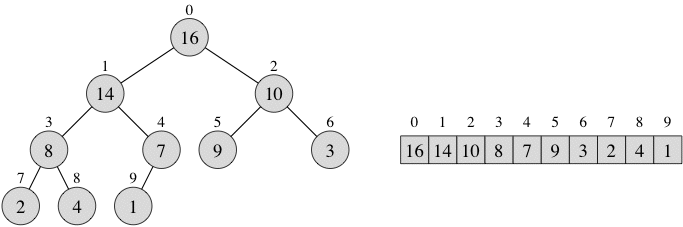
\includegraphics[width=\textwidth*13/16]{heaparray.png}
        \caption*{\emph{A max heap visualized as both a tree and an array.}}
    \end{figure*}

    \textbf{Binary trees} are trees where each node can have up to $2$ children.\\

    \textbf{full binary tree}: tree in which every node in the tree has exactly $0$ or $2$ children.\\

    \textbf{complete binary tree}: tree in which every level is completely filled with nodes \emph{except possibly} the last. Last level is filled from left to right. If bottommost level is not full, tree is \emph{nearly complete}.\\

    \textbf{height}: the height of a node $u$ is the number of \textbf{edges} on the longest downward path from $u$ to a leaf. The height of a leaf node is $0$.\\

    \underline{Binary Tree Properties}\\

    • If $T$ is a nonempty, full binary tree, then the number of leaf nodes in $T$ is one more than the number of internal nodes in $T$.\\
    • If $T$ is a binary tree of height $h$, the total number of leaves in $T$ is at most $2^h$.\\
    • If $T$ is a binary tree of height $h$, $T$ has at most $2^{h+1} - 1$ nodes.\\
    • If $T$ is a nearly complete binary tree of $n$ elements, the height of $T$ is $\lfloor \log n \rfloor$.\\

    \underline{Depth-First Traversals}\\

    \textbf{Preorder Traversal}: For a node $x$, print the value of $x$ first, then visit $left(x)$ and then $right(x)$.\\
    \textbf{Postorder Traversal}: For a node $x$, visit $left(x)$, $right(x)$, and then print the value of $x$.\\
    \textbf{Inorder Traversal}: For a node $x$, visit $left(x)$, print the value of $x$, and then visit $right(x)$.\\

    \underline{Breadth-First Traversals}\\

    \textbf{Level-Order Traversal}: Visit nodes by levels from left to right.\\

    %%%%%%%%%%%%%%%%%%
    %% BINARY HEAPS %%
    %%%%%%%%%%%%%%%%%%

    {\large \underline{Binary Heaps}}\\

    \emph{Partially Ordered}, satisfies heap property - parent is larger/smaller than any node in subtree (dep. on max/min-heap).\\
    
    \emph{Shape Property}, a binary heap is a \emph{nearly complete binary tree}.\\

    \emph{Array Implementation (1-Indexed)}, node $i$ has children at indices $2i$, $2i + 1$ and parent at $\lfloor i/2\rfloor$.\\

    \underline{Heap Construction.} Heaps can be constructed from an unsorted array in $O(n)$ time. A naive approach might use successive insertions into a heap, but this would result in $O(n \log n)$ time.\\
    
    The intuition behind this is that most of the nodes in a heap are at the bottom of the tree. As a result, these nodes can't be swapped very far down! Additionally, it turns out that not every set of swaps runs in $\Theta(\log n)$ time...\\
    
    Suppose for the sake of example that we have a max-heap with an underlying array $A$. We first arbitrarily fill $A$ with the elements we want to heapify. We define the \texttt{siftDown(i)} function as follows:

    \begin{framed}
    \begingroup
    \makeatletter
    \@totalleftmargin=-1.5cm
    \begin{verbatim}
        siftDown(A, i):
            m = A.heapsize
            while left(i) <= m:
                child = left(i)
                if right(i) <= m and 
                  A[left(i)] < A[right(i)]:
                    child = right(i)
                if A[i] < A[child]:
                    swap(A[i], A[child])
                else
                    return
    \end{verbatim}
    \makeatother
    \endgroup
    \end{framed}

    Under the assumption that the left and right subtrees of the $i$th vertex are valid max heaps, \texttt{siftDown} ensures that the subtree rooted at $i$ is also a valid max heap.

    \begin{framed}
    \begingroup
    \makeatletter
    \@totalleftmargin=-1.5cm
    \begin{verbatim}
        buildHeap(A):
            for i = floor(A.heapsize/2) downto 1:
                siftDown(A, i)
    \end{verbatim}
    \makeatother
    \endgroup
    \end{framed}

    \texttt{buildHeap} runs in $O(n)$ time. We start halfway in $A$ because the latter half of the heap are just the leaves (individual nodes are already heaps). Because of the shape property, the heap contains $2^{h-j}$ nodes with height $j$ at each level of the tree. A node at height $j$ can sift down at most $j$ levels. Counting in terms of the number of swap operations, we have at most $T(n) = \sum_{j=0}^h j 2^{h-j}$ swaps.\\

    Therefore, $$T(n) = \sum_{j=0}^h j2^{h-j} = \sum_{j=0}^h j\frac{2^h}{2^j} = n \sum_{j=0}^h \frac{j}{2^j}$$ since $n = 2^h$. (We can assume for simplicity that this is true.)

    $$T(n) = n\sum_{j=0}^h \frac{j}{2^j} \leq n\sum_{j=0}^\infty \frac{j}{2^j} = O(n)$$

    using the unbounded geometric series formula.\\\\

    \underline{Other Operations}\\

    Search for element in $O(n)$.\\

    Insertion in $O(\log n)$.\\

    Root peek in $O(1)$.\\

    Root removal in $O(\log n)$.\\

    \underline{Heapsort}. \texttt{Heapsort} sorts an input list in $\Theta(n\log n)$ time. It is an in-place but unstable sort. It converts the list to a heap first, and builds the sorted list from the right by extracting the root, swapping it with the last element in the heap, and sinking the new root.

    \begin{framed}
    \begingroup
    \makeatletter
    \@totalleftmargin=-1.5cm
    \begin{verbatim}
        heapsort(A):
            buildHeap(A)
            i = A.heapsize
            while i > 1:
                swap(A[i], A[1])
                i--
                siftDown(A, 1)
    \end{verbatim}
    \makeatother
    \endgroup
    \end{framed}

    The $\Theta(n\log n)$ time comes from running \texttt{siftDown} $n$ times.\\
    
    \textbf{Important: } Why is \texttt{heapsort} $\Theta(n\log n)$ and \texttt{buildHeap} not? In both functions we call \texttt{siftDown} at least $n/2$ times.\\

    A somewhat tongue-in-cheek answer - you can check the above math for \texttt{buildHeap}! More seriously, it is important to consider that for a particular node $i$ being sifted down, the total number of swaps will \textbf{not} be $\Theta(\log n)$. No work will be done for half of the nodes in the tree at the leaf-level, and as the height increases, the number of nodes that have to do more work decreases exponentially. (e.g. the root is the only node that might have to be swapped $\log n$
    times.)\\

    In contrast, in \texttt{heapsort}, at each iteration of the loop we extract the maximum of the heap and have to sift down a value at the \textbf{root} each time. As a result, the amount of comparisons \texttt{siftDown} will need is always going to be $\Theta(\log n)$. The tree will shrink as we remove elements, but it doesn't shrink nearly as fast! The height only decreases by $1$ once half of the nodes have been removed. \\

    \underline{Priority Queues}\\

    Min/max heaps can be used to implement a \texttt{PriorityQueue}. Each node in the heap contains a key and a value - where the key (priority) is used for the heap ordering and the value is associated with the given key. A heap-based \texttt{PriorityQueue} could implement a \texttt{changePriority(key, prio)} in $O(\log n)$ time.\\
    
    \emph{Caveat:} Java's implementation does \textbf{not} have this method. The only way to change an element's priority would be to remove it by value
    $O(n)$ and then re-insert it with a new key.\\

    \underline{Applications of Heaps}\\

    •Heapsort\\
    •$k$ smallest elements in an array.\\
    •Dijkstra's Algorithm\\
    •Prim's MST Algorithm\\

    %%%%%%%%%%%%%%%%%%%%%%%%%
    %% BINARY SEARCH TREES %%
    %%%%%%%%%%%%%%%%%%%%%%%%%
    {\large \underline{Binary Search Trees}}\\

    \textbf{BST Property}: the value in each node is larger than values in left subtree, and smaller than values in right subtree.\\

    Insertion, search, and delete operations then run in $O(h)$ time. Issue is that $h$ is not necessarily $\log n$.\\

    \textbf{Best Case}: Insertion, search, delete in $O(\log n)$.\\

    \textbf{Worst Case}: Insertion, search, delete in $O(n)$. Unbalanced tree (think of a spine, effectively a linked list.)\\

    \underline{Balanced Binary Search Trees}\\

    Because most of the operations on a BST run in time proportional to the tree height, keeping the tree's height minimal is optimal. A \textbf{self-balancing} BST minimizes its height given a sequence of arbitrary insertions and deletions.\\

    \textbf{2-3 Trees}\\

    A self-balancing tree where each node with children has either $2$ ($2$-node) or $3$ children ($3$-node). All leaves in a 2-3 tree are at the same level, and all data is kept in sorted order.\\
    
    A $2$-node satisfies the BST property. Suppose there is a $3$ node with keys $a, b$ s.t. $a < b$ and left child $L$, middle child $M$, and right child $R$. For all such nodes, $L, M, R$ are 2-3 trees of the same height, $a$ is greater than each element of $L$
    and less than or equal to each element in $M$, and $b$ is greater than each element in $M$ and less than or equal to each element in $R$.\\

    \underline{Search}: Operates much like binary search in a standard BST - with the addition that we can explore the the middle subtree of a $3$-node in our tree traversal.\\

    \underline{Insertion}: Search for the proper location of the key to insert and add it to the node. If the node is a $2$-node, then it becomes a $3$-node. If it is a $3$-node, it becomes a $4$-node with keys $a, b, c$ s.t. $a < b < c$. The $4$-node splits and the middle key $b$ moves up to the parent. This process is repeated upwards until the top is reached.\\

    \textbf{Red Black Trees}\\

    A self-balancing BST where each node is assigned the color red or black.\\

    \underline{Properties.}\\
    • A node is either red or black.\\
    • The root is always black or of negligible color.\\
    • If an internal node is red, then both of its children are black.\\
    • \emph{Every path from a given node to any leaves in its subtree contains the same number of black nodes, its \textbf{black height}.}\\

    The path from the root to the furthest leaf is no more than twice as long as the path from the root to the nearest leaf. Why?\\
    
    Because a red node must have black children, it is impossible to have two consecutive red nodes in a path from a node to its leaves. Therefore, the longest path contains at most $2*(\text{black height})$ nodes, alternating black and red. The shortest path contains at least $(\text{black height})$ nodes, all black. Given the property that every path from a
    particular node to its leaves contains the same number of black nodes, no path is more than twice as long as any other path.\\

    This property allows a red-black tree to remain roughly balanced at all times.

    \textbf{Left Leaning Red Black Trees}\\

    A modification to a standard red-black tree with the additional constraint that all red links (i.e. edge to a child red node) must be left edges except during insertion and removal.\\

    \underline{Search.} Exactly the same as BST search.\\

    \underline{Insertion.} Inserting an element in a LLRB starts off exactly like insertion in a BST by traversal. The element is added as a red node, and if any of the red-black tree properties are violated (e.g. two consecutive red nodes), a series of rotations or color flips are performed as depicted below.

    \begin{center}
    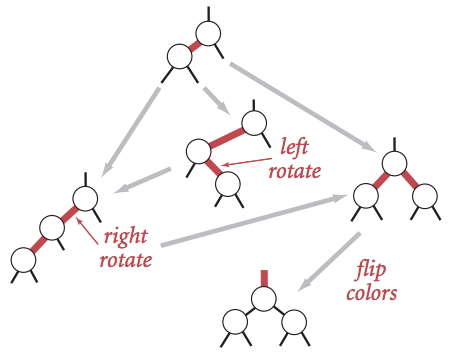
\includegraphics[width=\textwidth*2/5]{llrb.png}
    \end{center}

    \underline{Relationship with 2-3 Trees}. LLRBs provide an implementation for 2-3 trees. It turns out that a LLRB is isomorphic with a 2-3 tree, as demonstrated on the next page. Any node with a left leaning red child corresponds to a 3-node!\\

    \underline{Runtime Analysis.} It can be shown (but not here) that a red-black tree with $n$ internal nodes has a height of $O(\log n)$. Consequently, search runs in $O(\log n)$ time. For insertion, inserting the node takes $O(\log n)$ time. Additional work required to `fix' the tree upwards is proportional to $h$ and only requires $O(1)$ color flips or rotations. Therefore, insertion is $O(\log n)$ as well.

    %\underline{AVL Trees}\\

    %\textit{Self-balancing} BST, uses rotations.\\
    %Operations run in $O(\log n)$ time, even in worst case.\\
    %\textit{AVL Property} - each node's left/right subtrees differ in height by at most $1$.\\

    \end{multicols*}
    \newpage
    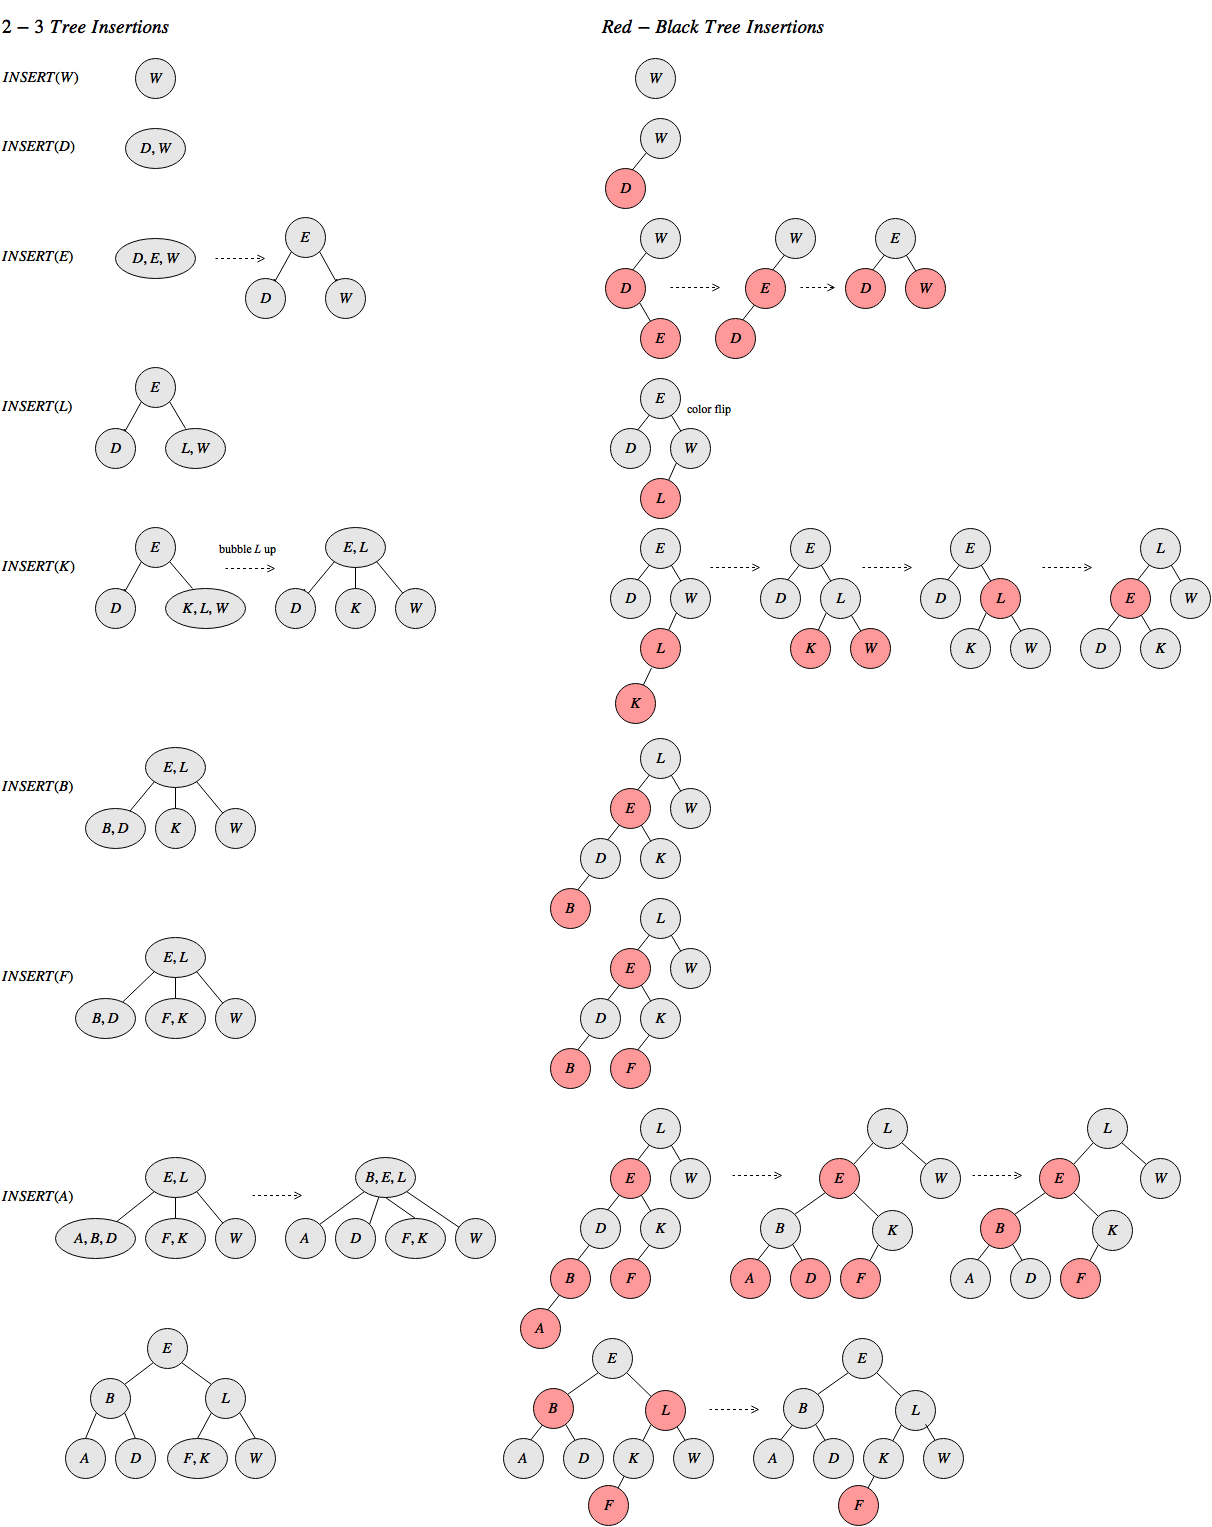
\includegraphics[width=\textwidth]{llrb23.png}
    \newpage
    \begin{multicols*}{2}

    %%%%%%%%%%%%%%%
    %% HASH MAPS %%
    %%%%%%%%%%%%%%%
    {\large \underline{Hash Maps}}\\

    Expected $O(1)$ lookup, insertion, removal.\\

    Implemented with an underlying array of size $m$ (number of buckets) and a particular hash function $h(\cdot)$.\\

    \underline{Simple Uniform Hashing Assumption}.\\ The basic assumption that a particular hash function $h(\cdot)$ will equally distribute elements into the table buckets. That is, the probability that two distinct keys $a, b$ will produce a collision is $$P(h(a) = h(b)) = \frac{1}{m}$$
    The SUHA gives that the \emph{load factor} of the hash table $\alpha$ is $$\alpha = \frac{n}{m}$$

    \underline{Hashing with Chaining}. Each array index contains a linked list of elements. When a collision occurs, append entry to end of the corresponding linked list (chain). The expected length of each chain is $\alpha$ under the SUHA. Lookup runs in expected $\Theta(\alpha + 1)$ - $1$ to compute the hash and $\alpha$ to search the chain. If $m > n$, this is effectively constant time. (Hence the need to resize the table if $n$ gets too large.)\\

    \underline{Linear Probing}. In the case of a collision, step forward by $i$ entries (wraparound to the beginning of the table if needed) until an empty spot is found. $h(i, k) = h(k) + i\mod m$. Often, step size $i=1$ is used. May lead to clustering, removal is tricky.\\

    \underline{Double Hashing}. Similar to linear probing, except the step size is no longer fixed but computed by another hash function. $h(i,k) = (h_1(k) + i\cdot h_2(k)) \mod m$.\\\\

    %%%%%%%%%%%%%%%%%%
    %% GRAPH THEORY %%
    %%%%%%%%%%%%%%%%%%
    {\large \underline{Graph Theory (CIS160 Review)}}\\
    
    $G = (V, E)$. Graphs consist of a vertex set $V$ and an edge set $E$. An edge $(u, v)$ connects two vertices $u, v$.\\

    \textbf{directed graph} (digraph): A directed graph adds an ordering to each edge. $(u, v) \in E$ indicates a directed edge from $u$ to $v$. The reverse edge $(v, u)$ may not necessarily be in $E$!\\

    \textbf{undirected graph}: An undirected graph does not have a notion of directed edges. $(u, v) \in E \implies (v, u) \in E$. Any directed graph can be turned into an undirected graph by bidirecting the edges.\\

    \textbf{walk}: A walk is a sequence of alternating vertices and edges where each edge's endpoints are the preceding and following vertices in the sequence. e.g. $(1,2), (2,4)$ (implicit vertices not shown)\\

    \textbf{connected graph}: In a connected graph, there is a path between every pair of vertices. A path is defined to be an open walk from $u$ to $v$ s.t. $u \neq v$.\\

    \textbf{connected component}: A connected component of an \emph{undirected graph} is a subgraph that is connected and has no edges to additional vertices in the supergraph.\\

    \textbf{strongly connected component}: A SCC of a digraph is a subgraph where there is a path between any pair of vertices in the subgraph.\\

    \textbf{subgraph}: A subgraph $G'$ of $G$ is formed such that $V_{G'} \subseteq V_G, E_{G'} \subseteq E_G$.\\

    \textbf{cycle}: A cycle in a graph is a walk of length at least $3$ s.t. the first and last vertices are the same (and no other vertices are repeated). e.g. $(1, 2), (2, 3), (3, 1)$ is a cycle. A graph that has no cycles is \emph{acyclic}.\\

    \underline{Trees}. A tree is an acyclic, connected graph. An acyclic graph $G$ is also called a \emph{forest}. A tree is therefore a connected forest, and a disconnected forest contains more than one tree.\\

    Given a tree $T$, for any two vertices $u, v \in V_T$, there is a unique path $u \leadsto v$. Conversely, if $G$ is a graph with the property that for any two vertices $u, v$, there is exactly one path $u \leadsto v$, then $G$ must be a tree.\\

    Any tree $T$ with $n \geq 1$ vertices has $n - 1$ edges, s.t. $|E| = |V| - 1$.\\

    \underline{Graph Representations}\\

    Graphs are used to model a variety of problems. They are well suited for modeling networks and dependencies. Think Google Pagerank, social networks, travelling salesman, course pre-requisites, etc! We represent graphs using a couple of data structures.\\

    \textbf{adjacency list}: Vertices are stored as objects, and each vertex has a set of adjacent vertices. Alternatively, edges can also be stored as objects, and each vertex would have a set of edges. An edge would then contain the incident vertices. Allows additional information to be associated with vertices. The graph would then store a set of all of the vertex/edge objects. \emph{Good for representing sparse graphs.} \\

    \textbf{adjacency matrix}: A 2D matrix/array in which the rows indicate source vertices and columns represent destination vertices. The value in the $i$th row and $j$th column indicates the weight of the edge $(i, j)$ or $0$ if there is no such edge. Only allows for one edge between each pair of vertices. Extra data must be stored externally. \emph{Good for representing dense graphs ($|E| \sim |V|^2$), or if $\Theta(1)$ edge lookup needed.}\\

    \textbf{Runtimes for Graph Operations}\\

    {\scriptsize \begin{tabular}{|c|c|c|}\hline
    &\textbf{Adjacency List}&\textbf{Adjacency Matrix}\\\hline
    Add Vertex&$O(1)$&$O(|V|^2)$\\\hline
    Add Edge&$O(1)$&$O(1)$\\\hline
    Delete Vertex&$O(|E|)$&$O(|V|^2)$\\\hline
    Delete Edge&$O(|E|)$&$O(1)$\\\hline
    Contains Edge $(u,v)$&$O(\text{deg}(u))$&$O(1)$\\\hline
    \end{tabular}}\\\\

    %%%%%%%%%%%%%%%%%%%%%%%%
    %% DEPTH FIRST SEARCH %%
    %%%%%%%%%%%%%%%%%%%%%%%%
    {\large \underline{Depth First Search}}\\

    Graph traversal. Explores vertices outwards from a source vertex $s$ by following each path from $s$ as far as possible before backtracking.\\

    \emph{Runtime}: $O(|V| + |E|)$

    \begin{framed}
    \begingroup
    \makeatletter
    \@totalleftmargin=-1.5cm
    \begin{verbatim}
        # Simple, recursive DFS.
        DFS(G, s):
            s.discovered = True
            for v in s.neighbors():
                if not v.discovered:
                    DFS(G, v)
    \end{verbatim}
    \makeatother
    \endgroup
    \end{framed}

    DFS may also be implemented \emph{iteratively} using a \texttt{Stack} to keep track of vertices to be visited.\\

    \underline{DFS Forests.*} A DFS traversal from a vertex $s$ builds a DFS tree rooted at $s$. To formally illustrate DFS-related concepts, we can write a more detailed version of DFS than shown above. We will assign a color with each vertex to indicate its status in the DFS.\\

    A vertex is WHITE if it has not been visited yet by the DFS. A vertex is GRAY if it has been discovered by DFS but is not finished because we are still exploring its children. A vertex is BLACK if all of its children have been explored and we are done with it.\\

    We also assign a vertex a parent field to indicate its parent in the DFS tree, as well as discovered and finished times.\\

    \newpage

    \begin{framed}
    \begingroup
    \makeatletter
    \@totalleftmargin=-1.5cm
    \begin{verbatim}
        #Builds a DFS-*forest* from G.
        DFS(G):
            for each vertex u in G.V:
                u.color = WHITE
                u.parent = null
            time = 0
            for each vertex u in G.V:
                if u.color is WHITE:
                    VISIT(u)

        VISIT(u):
            u.discovered = ++time
            u.color = GRAY
            for each vertex v in u.neighbors():
                if v.color is WHITE:
                    v.parent = u
                    VISIT(v)
            u.color = BLACK
            u.finished = ++time
    \end{verbatim}
    \makeatother
    \endgroup
    \end{framed}

    \underline{Parenthesis Theorem*}\\
    
    Note that a vertex $u$ is WHITE before time $u.d$, GRAY between times $u.d$ and $u.f$, and BLACK onwards. The discovery and finishing times for vertices have a \emph{parenthesis structure}. (e.g. if we denote discovery of a vertex $u$ with a `(u' and its finishing with a `u)', then the entire sequence of discoveries and finishings makes a balanced nested parenthetical expression).\\

    The \textbf{parenthesis theorem} says that in the DFS of a graph $G$, for any two vertices $u, v$, exactly one of the following holds. ($d$ - discovered, $f$ - finished)\\

    • the intervals $[u.d, u.f]$ and $[v.d, v.f]$ are disjoint (don't overlap), and neither $u$ nor $v$ is a descendant of the other in the DFS forest\\
    • the interval $[u.d, u.f]$ is contained entirely within the interval $[v.d, v.f]$, and $u$ is a descendant of $v$ in a DFS tree\\
    • the interval $[v.d, v.f]$ is contained entirely within the interval $[u.d, u.f]$, and $v$ is a descendant of $u$ in a DFS tree

    \underline{Edge Classification*}\\

    Using DFS, we can also classify the edges of a graph into the following categories:\\

    \textbf{tree edge} - edges in the DFS forest. An edge $(u, v)$ is a tree edge if $v$ was first discovered by exploring $(u, v)$.\\

    \textbf{back edge} - edges $(u, v)$ connecting a vertex $u$ to an ancestor $v$ in a DFS tree. Self-loops are also back edges.\\

    \textbf{forward edge} - nontree edges $(u, v)$ connecting a vertex $u$ to a descendant $v$ in a DFS tree. (e.g. $v$ is a grandchild of $u$ and there is an edge $(u, v)$).\\

    \textbf{cross edge} - all other edges. Can go between vertices in the same DFS tree so long as one vertex is not an ancestor of the other, or can go between vertices in different DFS trees.\\

    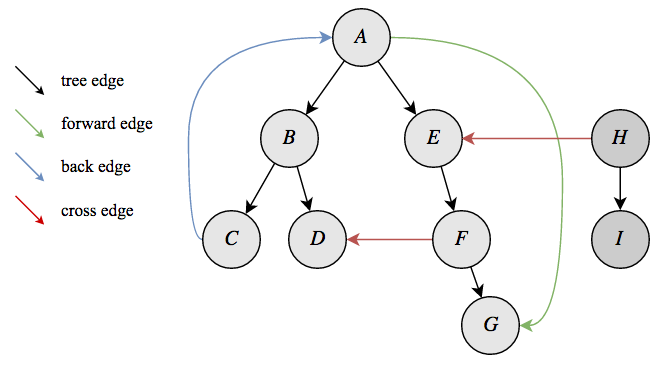
\includegraphics[width=\textwidth/2]{edgeclassification.png}

    \emph{Shown above is the graph $G$, with the edges recolored to show the edge classification after running DFS. Slightly different shades of gray are used to identify separate DFS trees in the forest.}\\

    When we first explore an edge $(u, v)$, the color of $v$ lets us classify the edge:\\

    • WHITE indicates a tree edge\\
    • GRAY indicates a back edge\\
    • BLACK indicates a forward/cross edge (forward if $u.d < v.d$ and cross if $u.d > v.d$)

    \textbf{Theorem.} In a DFS of an undirected graph $G$, every edge of $G$ is either a tree edge or a back edge. That is, a DFS of an undirected graph can not yield forward or cross edges.\\
    
    Why? Imagine that for the sake of contradiction when visiting a vertex $u$ you explore an edge $(u, v)$ such that $v$ is already colored BLACK. This is not possible! If $v$ is colored BLACK, then it must have already explored all of its edges, which includes $(v, u)$ in an
    undirected graph.\\

    \textbf{Lemma.} A directed graph is acylic iff a DFS yields no back edges.\\

    %\underline{White-Path Theorem}: In a DFS forest of a graph $G$, a vertex $v$ is a descendant of vertex $u$ iff at the time $u.d$ that the search discovers $u$, there is a path from $u$ to $v$ consisting entirely of white vertices.\\

    \underline{Applications}\\

    • Find a path from $s$ to $t$ in graph and length/cost of path.\\
    • Build DFS tree rooted at $s$.\\
    • Topological Sorting.\\
    • Bipartite testing.\\
    • Cycle detection.\\
    • Find SCCs of graph.\\

    %%%%%%%%%%%%%%%%%%%%%%%%%%
    %% BREADTH FIRST SEARCH %%
    %%%%%%%%%%%%%%%%%%%%%%%%%%
    {\large \underline{Breadth First Search}}\\

    Graph traversal. Explores vertices outwards from a source vertex $s$ in a \emph{level-order} fashion, i.e. suppose a vertex $t$ has shortest distance $d$ to $s$. $t$ is not explored until all vertices with shortest distance $d-1$ are explored first. Similar in logic to Prim's MST and Dijkstra's shortest path algorithms - priority based graph searching.\\

    \emph{Runtime}: $O(|V| + |E|)$\\

    BFS decomposes a graph $G$ into layers $L_i$ s.t. the shortest path from $s$ to each of the vertices in $L_i$ is of length $i$. $L_0 = \{s\}$. Given layers $L_0, L_1, \dots, L_j$, then $L_{j+1}$ is the set of vertices that are not in a previous layer and that have an edge to some vertex in layer $L_j$.

    \emph{Theorem for Non-BFS Edges.*} Choose $x \in L_i$ and $y \in L_j$ s.t. $(x, y) \in E_G$. Then $|j-i| \leq 1$. That is, edges of $G$ that do not appear in the BFS tree connect nodes either in the same layer (cross edges) or in adjacent layers (tree edges). A BFS can not produce forward edges. In an undirected graph, it can also not have backward edges. \\

    BFS generates a breadth-first search tree based at $s$ - effectively a shortest path tree. That is, it finds the paths from $s$ to other vertices that use a minimal number of edges. For an unweighted graph this solves the shortest path problem! (But not necessarily for a weighted graph).\\

    \begin{framed}
    \begingroup
    \makeatletter
    \@totalleftmargin=-1.5cm
    \begin{verbatim}
        # Simple, iterative BFS.
        BFS(G, s):
            Q = {s}
            s.visited = True
            while Q is not empty:
                cur = Q.dequeue()
                for vertex v in cur.neighbors():
                    if not v.visited:
                        v.visited = True
                        Q.enqueue(v)
    \end{verbatim}
    \makeatother
    \endgroup
    \end{framed}

    \underline{Applications}\\
    • Shortest paths from $s$ to all vertices on unweighted graph.\\
    • Build BFS tree rooted at $s$.\\
    • Find depth of longest path rooted at $s$.\\
    • Bipartite testing.\\
    • Cycle detection.\\

    \begin{figure*}[t]
        \centering
        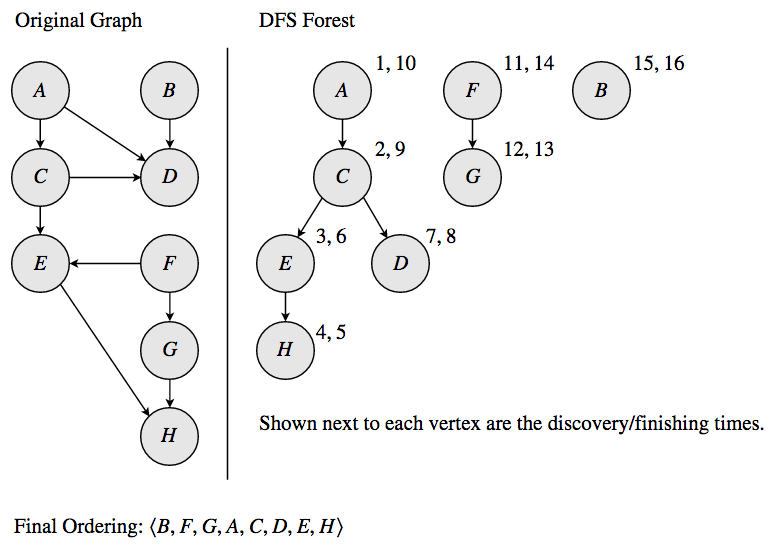
\includegraphics[width=\textwidth*5/8]{toposort.png}
        \caption*{\emph{An example of toposort on an input graph $G$.}}
    \end{figure*}

    \underline{BFS vs. DFS?}\\
    
    Although the asymptotic complexities of BFS and DFS are identical, the ways they build their respective search trees are very different! If the graph is very large, the DFS tree is deep, and searched for items are rare, DFS may time out/take a long time. BFS could be faster. If the tree is too deep, the DFS search depth might have to be restricted (iterative deepening). If the searched for items are close to the root of the search tree, BFS could be better! If a tree is very wide, BFS could run out of memory. If the searched for items are deep in the
    tree, BFS could also take too long.\\

    {\large \underline{Topological Sort}}\\

    Generates a linear ordering of the vertices of a DAG $G$. Labels vertices such that all edges between vertices point towards higher labeled vertices. For each edge $(u, v)$ in $G$, $u$ appears before $v$ in the ordering. That is, all edges point forward.\\

    A topological sort can be generated for a graph by simply running a DFS on $G$ and \emph{prepending} the vertex labels to a list whenever a vertex is finished (colored black). That is, the vertices are placed in reverse order of finish times. The runtime for this algorithm is $\Theta(|V| + |E|)$, just like a standard DFS.\\

    A graph can have \emph{multiple} topological orderings! This should be obvious - different starting points can be used for the DFS during iteration, each of which will generate a different ordering.\\

    \underline{Applications}.\\
    • Instruction scheduling (or any sort of dependency network, e.g. in the C linker)\\
    • Shortest paths in a weighted DAG\\

    {\large \underline{Kosaraju's Algorithm}}\\

    Linear time algorithm to find the strongly connected components (SCCs) of a digraph.\\

    \emph{Observation}: The transpose graph $G^T$ has the exact same SCCs as $G$. We define $G^T$ to be the same graph as $G$ with every edge's direction reversed. $G^T = (V, E^T)$ s.t. $E^T = \{(v,u) | (u,v) \in E\}$.\\

    \emph{Computing $G^T$:} For an adjacency matrix representation, computing $G^T$ is as simple as taking the transpose of the matrix. For an adjacency list, one has to iterate through each vertex's neighbors and add the reversed edge to a new graph representation.\\

    \underline{Algorithm.}\\

    Initialize an empty stack $S = \{\}$. Run a DFS on $G$ to generate a DFS forest. Whenever a vertex is finished, push it onto $S$. Compute the transpose graph $G^T$. Initialize a label variable $l = 1$. Pop off the first vertex $u$ from $S$ and label it with $l$. Run a single DFS from $u$ - for each visited vertex, label it with $l$. Once the DFS has finished, increment $l$. Repeat until $S$ is empty. If a vertex removed from $S$ already has a label, skip
    it.\\

    \underline{Runtime.}\\
    
    The stack in the algorithm is used to generate a \emph{reverse postordering} on the graph $G$. The runtime of this algorithm is $\Theta(|V|+|E|)$ time when $G$ is represented as an adjacency list. If $G$ is represented as an adjacency matrix, the algorithm runs in $\Theta(|V|^2)$ time due to the cost of transposing the matrix.\\

    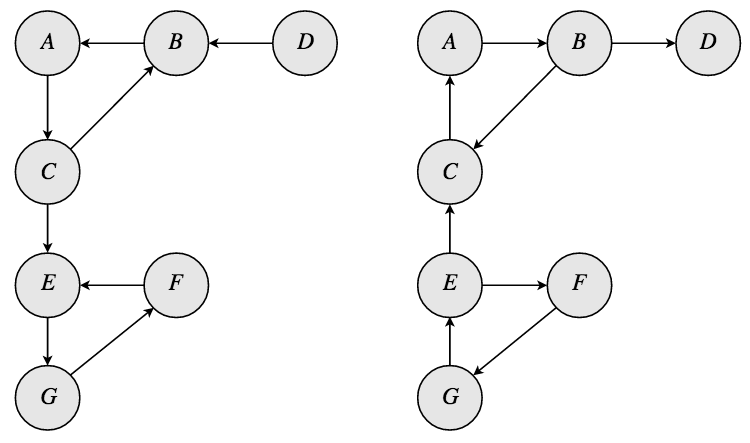
\includegraphics[width=\textwidth*1/2]{kosaraju.png}\\

    \underline{Example}.\\

    Shown above are the graphs $G$ and $G^T$. Suppose we run Kosaraju's on $G$. We first generate a reverse postordering $\langle D, A, C, E, G, F, B \rangle$. We then run a DFS on $G^T$ starting from $D$. This DFS gives us $\langle D \rangle$. Doing a DFS from $A$, we get $\langle A, C, B \rangle$ - these are in one SCC. Doing a DFS from $E$, we get the $\langle E, F, G \rangle$ (we don't explore $C$ because it's already been labeled). The DAG kernel graph is shown next:\\

    \begin{centering}
        \hspace{50pt}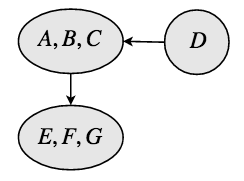
\includegraphics[width=\textwidth*1/4]{dagkernel.png}\\
        \emph{The DAG Kernel graph for $G$. SCCs are contracted into a single vertex.}\\
    \end{centering}\mbox{}\\

    %%%%%%%%%%%%%%%%%%%%%%%%%%%%
    %% MINIMUM SPANNING TREES %%
    %%%%%%%%%%%%%%%%%%%%%%%%%%%%
    {\large \underline{Minimum Spanning Trees}}\\

    Given an undirected, connected graph $G$, a tree $T$ is a spanning tree if it \emph{spans} $G$ (s.t. it contains all of the vertices of $G$) and if its edges are all contained in $G$.\\

    \textbf{minimum spanning tree} - a MST is a spanning tree of minimal total weighting for its edges.\\
    
    \underline{MST Multiplicity.} A graph $G$ can have multiple MSTs. For example, if all of the edge weights of a graph $G$ are the same, every spanning tree of the graph is minimum.\\

    \underline{MST Uniqueness.} If each edge in a graph $G$ has a distinct weight then $G$ has exactly one, unique MST.\\

    \underline{Cycle Property.} For any cycle $C$ in the graph, if the weight of an edge $e \in C$ is larger than the individual weights of all other edges in $C$, then this edge can not belong in an MST.\\

    \underline{Cut Property.*} A \emph{cut} of a graph $G$ is a partitioning of its vertices into two disjoint subsets. For any cut $C$ in the graph, if the weight of an edge $e$ of $C$ is strictly smaller than the weights of all other edges of $C$, then this edge belongs to all MSTs of $G$.\\

    \underline{Minimum-Cost Edge.} If the edge of a graph with the minimum cost is unique, then this edge is included in any MST.\\

    \underline{Applications}\\

    • Spanning Tree Protocol (STP) for Ethernet networks. Used to generate a topology for a network that contains no loops! A network with loops can result in the same network broadcast messages circulating around the network, consuming network resources.\\
    • Widest path problem for undirected graphs.\\
    • Network Design\\
    • Lots of other complicated things (see Wikipedia).\\

    %%%%%%%%%%%%%%%%%%%%%%%%%
    %% KRUSKAL'S ALGORITHM %%
    %%%%%%%%%%%%%%%%%%%%%%%%%
    {\large \underline{Kruskal's Algorithm.}}\\

    Finds a minimum spanning tree for a connected weighted graph.\\

    \underline{Algorithm.} Create a union-find forest $F$ for each vertex and an empty set $S$. Create a min-heap $Q$ containing all of the edges with the weights as keys. While $Q$ is not empty and $F$ is not a spanning tree, call EXTRACT-MIN on $Q$. Let $(u, v)$ be the removed edge. If $(u, v)$ connects two different components in $F$, then add it to $S$ and call UNION($u$, $v$) on $F$. When finished, return $F$ and $S$.\\

    When the algorithm is complete, $F$ is either a single component and $S$ is a MST. Otherwise, $F$ has multiple components and represents a minimum spanning forest.\\

    \underline{Runtime.} Kruskal's runs in $O(E \log E)$ time. The bottleneck operation in Kruskal's is the task of 'sorting' the edges (accomplished here via min-heap). We perform at most $O(E)$ removals from the min-heap when attempting to add new vertices to the spanning tree, and for each attempt we have an $O(\alpha(V))$ operation for FIND and UNION. Since $O(\alpha(V)) \in O(\log V) \in O(\log E)$, this gives us $O(E \log E)$ time.\\

    %%%%%%%%%%%%%%%%%%%%%%%
    %%% PRIM'S ALGORITHM %%
    %%%%%%%%%%%%%%%%%%%%%%%
    {\large \underline{Prim's Algorithm.}}\\

    Finds a minimum spanning tree for a connected weighted graph. Grows the MST from a single vertex by adding minimum weight edges to non-tree vertices.\\

    \underline{Algorithm.} Create a tree $T$ from any vertex $v$ in $G$. In increasing order of weight, pick the next minimum-weight edge that connects any vertex not in $T$ to a vertex in $T$. Repeat until all edges have been exhausted or $T$ spans $G$.\\

    We have two approaches to ``picking the next minimum-weight edge connecting a tree vertex to a non-tree vertex."\\

    \emph{Lazy approach}: Store edges in a min-heap with the weights as the keys. Initialize the min-heap $Q$ to contain all edges from $v$. Whenever a new vertex $u$ is added to $T$, add to $Q$ all edges that connect $u$ to a vertex not yet in the tree. If a call to EXTRACT-MIN yields an edge that is ineligible (connects two vertices in the tree), skip it.\\

    \emph{Eager approach}: Initialize a table of size $|V|$, $minEdges$. For the vertex with label $v$, $minEdges[v]$ will contain the shortest edge connecting the MST to a non-tree vertex. Initialize the min-heap $Q$ to contain the starting vertex $s$ with $0$ as the edge weight. While the queue is not empty, call EXTRACT-MIN. Let $u$ be the vertex obtained from EXTRACT-MIN. For each edge $(u, v)$ with edge weight $w$, if $w < minEdges[v].weight$, update $minEdges[v] = (u,v)$. Then,
    if $v \in Q$, update the priority of $v$ in $Q$ to be $w$ with DECREASE-KEY. Otherwise, add $v$ to $Q$ with priority $w$. When the loop is finished, return a set of all of the edges in $minEdges$ - this is the MST.\\

    The main distinction is that the lazy approach considers all edges in the graph (in the min-heap), whereas the eager one only considers the lightest edge weight connecting each vertex not in the tree. This means that the min-heap used for the lazy approach will be of size $O(E)$ vs. $O(V)$ in the eager approach.\\

    Lazy Prim's runs in worst case $O(E \log E)$ with $O(E)$ space since we add and consider all edges in the min-heap. Eager Prim's runs in worst case $O(E\log V)$ with $O(V)$ space, as we might call DECREASE-KEY for each edge (as well as make $V$ calls to EXTRACT-MIN).\\

    %$\alpha(m,n) = \min\{i \geq 1\;:\;A(i,\floor{m/n}) > \log n\}$

    %%%%%%%%%%%%%%%%%%%%%%%%%%
    %%% WIDEST PATH PROBLEM %%
    %%%%%%%%%%%%%%%%%%%%%%%%%%
    {\large \underline{Widest Path Problem*}}\\

    Given two vertices $s, t$, find the maximum capacity path $s \leadsto t$ such that the smallest weight (lightest) edge on the path is maximal across all paths from $s$ to $t$.\\

    It is often useful to think of edge weights in a graph as \emph{capacities} for flow. For example, imagine that a graph $G$ represented a supply-trade network between cities. For any pair of cities, either can send goods to the other at a rate limited by the number of trains between them (edge weights). When sending goods on a path between two cities, the total amount of goods that can be sent is limited by the edge that has the smallest number of trains (smallest
    weight).

    \begin{center}
    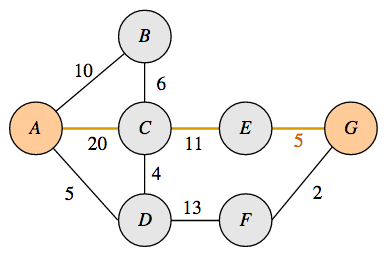
\includegraphics[width=\textwidth*3/8]{widestpath.png}\\
    \emph{The widest path from $A$ to $G$ is colored in orange. The bottleneck (lightest) edge on the path is $(E, G)$.}
    \end{center}

    In the above figure, there are multiple paths from $A$ to $G$, such as $A\leadsto D \leadsto F \leadsto G$. However, this is not the widest path, as the lightest edge on this path is $(F, G)$ with a capacity of $2$.\\

    For an \emph{undirected graph} $G$, the widest path can be computed by finding the maximum spanning tree (tree whose weight is maximal among all other spanning trees), and finding a path from $s$ to $t$ in said tree.\\

    \underline{Algorithm.} Suppose we are given a graph $G$ with source vertex $s$ and destination vertex $t$. Compute the graph $G'$ by multiplying all of the edge weights of $G$ by $-1$. (i.e. if $G$ has weight function $c_G : E \rightarrow \mathbb{R^{+}}$, $c_{G'} = - c_{G}$). Run Kruskal's algorithm to compute the minimum spanning tree of $G'$, $T$. Then run a BFS from $s$ in $T$ to compute the path from $s$ to $t$. Return this path.

    \begin{center}
    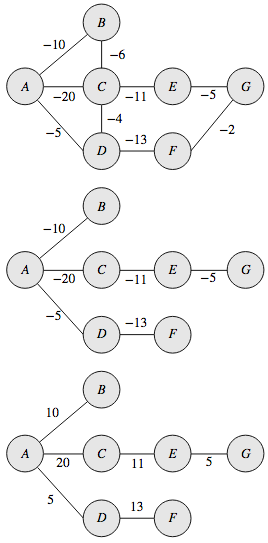
\includegraphics[width=\textwidth*5/16]{widestpath2.png}\\
    \emph{Computing the maximum spanning tree of $G$ by negating the edges.}
    \end{center}

    \newpage

    The maximum spanning tree can be computed by negating the edge weights and finding the minimum spanning tree of the modified graph. Since by definition, a tree contains exactly one path between each pair of vertices $u, v$, the unique path between $s$ to $t$ in the maximum spanning tree is the widest path.\\

    \underline{Runtime.} The runtime of this algorithm is $O(E \log E)$ - the cost of computing the minimum spanning tree with Kruskal's. BFS is linear $O(V + E)$, and the cost of computing the negative edge weights is $O(E)$ - both of which are $O(E \log E)$.\\

    \underline{Applications.}\\

    • Finding an end to end path in a computer network with maximum bandwidth.\\
    • Winner of a multiway election.\\
    • Max flow computation (CIS320, Network Flows).\\

    {\large \underline{Dijkstra's Algorithm}}\\

    Finds the shortest path from a source vertex $s$ to all other vertices in a weighted graph with \emph{non-negative edge weights}. Greedily solves the \emph{single-source shortest path} problem.\\

    \underline{Algorithm.} Initialize a table $d[v]$ to contain the minimum distances seen thus far from $s$ to other vertices. Set $d[v] = \infty$ for all $v \neq s$, and set $d[s] = 0$. Initialize another table $p[v]$ to contain the previous vertex before $v$ in the shortest path from $s$ to $v$. Set $p[v] = \text{null}$ for all $v$. Initialize a min-heap $Q$ to contain all of the vertices where the keys (priorities) are the distances in $d$. While $Q$ is not empty, call EXTRACT-MIN and let $u$ be the vertex obtained. For each edge $(u, v)$ with edge weight $w$, if $d[u] + w < d[v]$, update $d[v] = d[u] + w$ and
    update the priority of $v$ in $Q$ to be this new value with DECREASE-KEY. Set $p[v] = u$. (This is the \emph{edge relaxation} step!). When finished, return $d$ and $p$.\\

    The shortest path from $s$ to a vertex $v$ can then be computed by following the values in $p$ in reverse.\\

    \underline{Runtime.} $O((V+E)\log V)$. The min-heap is of size $V$, and we perform $V$ EXTRACT-MIN operations and at most $E$ DECREASE-KEY operations, each of which are $O(\log V)$.\\

    \underline{Example.}

    \begin{center}
    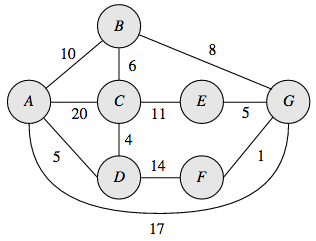
\includegraphics[width=\textwidth*3/8]{dijkstras.png}\\
    \end{center}

    Shown above is the undirected weighted graph $G$. Suppose we run Dijkstra's algorithm on $G$ from the vertex $A$. We denote the steps in a table:

    \begin{center}
    \begin{tabular}{|c|c c c c c c c c|}\hline
    $A$&$0$&$\mathbf{0}$&-&-&-&-&-&-\\
    $B$&$\infty$&$10$&$10$&$10$&$\mathbf{10}$&-&-&-\\
    $C$&$\infty$&$20$&$9$&$\mathbf{9}$&-&-&-&-\\
    $D$&$\infty$&$5$&$\mathbf{5}$&-&-&-&-&-\\
    $E$&$\infty$&$\infty$&$\infty$&$20$&$20$&$20$&$20$&$\mathbf{20}$\\
    $F$&$\infty$&$\infty$&$19$&$19$&$19$&$18$&$\mathbf{18}$&-\\
    $G$&$\infty$&$17$&$17$&$17$&$17$&$\mathbf{17}$&-&-\\\hline
    \end{tabular}
    \end{center}

    Each column represents the entries of $d$ at each iteration of the while loop in Dijkstra's algorithm, and each row depicts how the values of $d[i]$ change for the $i$th vertex. A bolded value indicates that we have just removed that vertex from the min-heap. The dashes indicate that the value of $d[v]$ for a particular vertex will no longer change in the algorithm.\\

    \underline{Greedy Algorithms*.}\\
    
    Dijkstra's algorithm is a greedy algorithm, an algorithm that tries to solve a problem by making \emph{locally optimal} choices at each stage. A greedy algorithm may not necessarily produce an optimal solution (a global one).\\

    \underline{Failure for Negative Edge Weights.}\\
    
    Dijkstra's algorithm may work for some graphs that contain negative edge weights, but not all. \\

    \begin{center}
    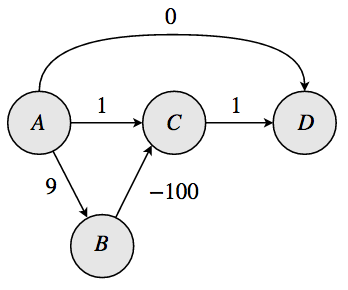
\includegraphics[width=\textwidth*3/8]{dijkstrasnegative.png}\\
    \emph{An example of a graph where Dijkstra's will fail to find the shortest path.}
    \end{center}

    Let us consider the graph shown above. Running Dijkstra's algorithm from $A$ will fail to produce the correct shortest paths.

    \begin{center}
        \begin{tabular}{|c| c c c c c|}\hline
        $A$&$0$&$\mathbf{0}$&-&-&-\\
        $B$&$\infty$&$9$&$9$&$9$&$\mathbf{9}$\\
        $C$&$\infty$&$1$&$1$&$\mathbf{1}$&$-91$\\
        $D$&$\infty$&$0$&$\mathbf{0}$&-&-\\\hline
        \end{tabular}
    \end{center}

    Observe that while the shortest distance from $A$ to $C$ is correct, the shortest distance from $A$ to $D$ is given as $0$ even though the actual value is $-90$.\\

    \underline{Failure for Negative Cycles.}\\

    Dijkstra's will further fail on graphs with negative cycles reachable from $s$ (a cycle where the total weight is negative). A negative cycle indicates that a shortest path does not exist, since the total weight lowers each time the cycle is traversed.\\

    %Greedy algorithm that uses \textit{edge relaxation} at each iteration to approach an optimal solution.\\

    {\large \underline{DAG Shortest Paths}}\\

    Linear time $\Theta(V + E)$ algorithm to solve single source shortest paths in a DAG.\\

    \underline{Algorithm.} Topologically sort the DAG $G$ to get a linear ordering $L$. Initialize a table $d[v]$ to contain the minimum distances seen thus far from the source vertex $s$. Set $d[v] = \infty$ for all $v \neq s$ and set $d[s] = 0$. For each vertex $u$ in the ordering $L$, iterate through each of its outward edges $(u, v)$ with weight $w$. If $d[u] + w < d[v]$, relax $d[v] = d[u] + w$. When finished, return $d$.\\

    \underline{Runtime.} The runtime of this algorithm is $\Theta(V + E)$. The topological sort runs in $\Theta(V + E)$ time, initializing $d$ takes $\Theta(V)$ time, and each iteration of the inner for loop takes $\Theta(1)$ time. Consequently, in an adjacency-list representation the for loops run in $\Theta(E)$ time. The for loop relaxes each edge exactly once.\\

    {\large \underline{Bellman-Ford Algorithm}}\\

    $O(VE)$ time algorithm solving single-source shortest paths even when a graph contains negative weights. (Negative cycles still don't work, but this algorithm can detect them.)\\

    \underline{Algorithm.} Initialize a table $d[v]$ to contain the minimum distances seen thus far from the source vertex $s$. Set $d[v] = \infty$ for all $v \neq s$ and set $d[s] = 0$. Run a for loop $V - 1$ times. In each iteration, iterate through each edge $(u, v) \in E$ with weight $w$. If $d[u] + w < d[v]$, relax $d[v] = d[u] + w$. After this iteration is done, iterate through each edge $(u, v) \in E$ with weight $w$. If $d[u] + w < d[v]$, then we have a negative cycle.
    Otherwise, return $d$.

    \underline{Runtime.} Initializing $d$ takes $\Theta(V)$ time, and each of the $|V| - 1$ iterations of the first outer for loop runs in $\Theta(E)$ time since we iterate through the entire edge set. The last for loop runs in $O(E)$ time (Big-Oh because it can terminate early), and consequently we have $O(VE)$ total time.\\

    {\large \underline{Counting Sort}}\\

    ``Linear" time \emph{stable} sorting algorithm for integers or strings. \emph{Not} a comparison sort. Often used as a subroutine in radix sort (which is why it's important that this algorithm is stable).\\

    \begin{framed}
    \begingroup
    \makeatletter
    \@totalleftmargin=-1.5cm
    \begin{verbatim}
        Countingsort(A, k):
            output = new int[A.length]
            C = new int[k]  # initially zeroes
            for j = 0 to A.length-1:
                C[A[j]]++;  
            # C[i] contains num elements = i
            for i = 0 to k-1:
                C[i] = C[i] + C[i-1]
            # C[i] contains num elements <= i
            for j = A.length-1 downto 0:
                output[C[A[j]]] = A[j]
                C[A[j]]--
            # put each i in A in their sorted order
            return output
    \end{verbatim}
    \makeatother
    \endgroup
    \end{framed}

    In the above, $k$ indicates the maximum value of an element in the input array $A$. $C$ is an auxiliary array used to store the indices of where an element $i \in A$ should go in the sorted array.\\

    \underline{Runtime.} Runs in $\Theta(n + k)$ time. If $k = O(n)$, then counting sort runs in $\Theta(n)$ time.\\


    {\large \underline{Radix Sort}}\\

    Idea: If the input list contains numbers/strings of constant length, by sorting elements with respect to each digit/character, one can sort the entire list in linear time.\\

    \underline{LSD Radix Sort}\\

    \emph{Algorithm.} Suppose we are given an array $A$ that contains strings/integers with $d$ characters/digits. Run a for loop from $i = 1$ to $d$. Use the \emph{stable} counting-sort to sort $A$ with respect to the $i$th least significant character/digit and update $A$. Return $A$.\\

    \emph{Runtime.} The runtime of this algorithm is $\Theta(d(n+k))$ time, where $k$ is the \emph{radix} of the input (i.e. each digit can take on $k$ values). When $d$ is constant and $k = O(n)$, radix sort runs in \emph{linear time}.\\

    \emph{Example.}

    \begin{center}
    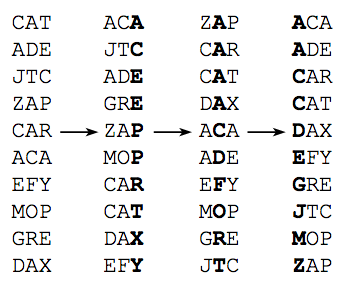
\includegraphics[width=\textwidth*2/5]{lsdradix.png}
    \end{center}

    Shown above is an example progression of radix sort. Each column represents one iteration of the for loop. Note that when sorting by the $2$nd characters, the relative ordering of the strings ZAP, CAR, CAT, and DAX are still preserved. Because counting-sort is stable, the ordering we get from sorting on the lower digits remains.\\

    \emph{Sorting Optimality.*} Note the following: given $n$ $b$-bit numbers and any positive integer $r \leq b$, radix sort correctly sorts these numbers in $\Theta(\frac{b}{r}(n+2^r))$ time using the $\Theta(n + k)$ time counting sort as a subroutine.\\
    
    For example, suppose that we have $32$-bit words that have four $8$-bit digits, s.t. $b = 32, r = 8$. Then the radix is $k = 2^r = 256$, and $d = \frac{b}{r} = 4$.\\

    Then we have $\Theta(d(n+k)) = \Theta(\frac{b}{r}(n+2^r))$. This indicates that given values of $n$ and $b$, $r$ must be chosen intelligently to maintain an optimal $\Theta(n)$ runtime. If $b < \lfloor \log n \rfloor$, then choosing any $ r \leq b$ will yield a $\Theta(n)$ runtime. Otherwise, if $b \geq \lfloor \log n \rfloor$, then choosing $r = \lfloor \log n \rfloor$ yields $\Theta(\frac{bn}{\log n})$. (Recall the constraint that $r \leq b$.)\\

    Often, $b = O(\log n)$. Picking $r \approx \log n$ yields a $\Theta(n)$ runtime. Compared to quicksort's expected $\Theta(n\log n)$ runtime, this might seem optimal! However, the hidden constant factors are different. This means that while counting sort might make less passes over the $n$ input keys than quicksort, it might spend more time on each one. Testing in practice would be the only way to determine relative optimality of the sorts. Additionally, radix sort with counting sort
    as a subroutine is \emph{not} in-place! If this is needed, a different in-place sorting algorithm would be required.\\

    \underline{MSD Radix Sort}\\

    \emph{Algorithm.} Perform a modified counting sort on $A$ with respect to the most significant digit (first character) that also returns the array $C$. Using the counts given in $C$, partition $A$ into subarrays $A_1, A_2, \dots A_k$, where $A_i$ contains keys whose first MSD is $i$. (Numbers used for subscripts, but could also be characters). Recursively call sort on each subarray $A_i$ starting from the next MSD. When finished, rejoin the subarrays in sorted order and
    return.\\

    \emph{Runtime.} The runtime of the MSD radix sort is still $\Theta(d(n+k))$. \emph{However}, the overhead is significantly higher than the LSD radix sort. Each recursive function call needs an additional array $C$. Additionally, the number of recursive calls grows \textbf{fast} - this will blow out the call stack!\\

    \emph{Insertion Sort Fallback.} To avoid the issue of having an obscene amount of recursive calls for small subarrays - MSD radix sort can be modified to switch to insertion sort once at some arbitrary $i$th character (which can be experimentally determined). The benefit of insertion sort here is that it runs in linear time for already sorted lists and has low overhead for small arrays despite its quadratic worst case runtime.\\
    

    {\large \underline{Tries} (Placeholder)}\\

    •Each node can have $k$ children, where $k$ is the alphabet size.\\
    •Node represents a 'fragment' of key in the trie.\\
    •Useful for dictionaries/associative arrays.\\
    •Space usage can be improved with compression (Patricia trie).\\

    {\large \underline{Huffman Encoding}}\\

    Encoding scheme where more frequent characters have shortest encoding. A type of optimal \emph{prefix code} - no code word in a code system is the prefix of another codeword! (e.g. a case where `A' - 01 and `B' - 010 can never happen.)\\

    Represented with Huffman tree, where left/right in traversal corresponds to a $0/1$ in the encoding.\\

    \underline{Tree Construction}\\
    
    The Hufmann encoding tree is generated given an alphabet and its corresponding probability distribution (frequencies).\\

    \emph{Algorithm.} Suppose you are given an alphabet $A = \{c_1 : f_1, c_2 : f_2, \dots, c_m : f_m\}$, where $c_i$ indicates the $i$th character and $f_i$ the frequency. Initialize a min-heap $Q$. Initialize a node $n_i$ for each character $c_i$, where $i = 1\dots m$.\\
    
    For two nodes $n_i, n_j$, $n_i < n_j$ if $f_i < f_j$. If $f_i = f_j$, then $n_i < n_j$ if $c_i < c_j$. If either $n_i$ or $n_j$ (or both) are internal nodes ($c_i = $NIL or $c_j = $NIL), $n_i < n_j$ if $i < j$, i.e. $n_i$ was created first.\\

    Initialize a time variable $t = m+1$. Add each node to $Q$. While $Q$ has at least two elements, call EXTRACT-MIN twice. Let $x, y$ be the retrieved nodes in order of removal, i.e. $x < y$. Initialize a new node $n_t$ such that $n_t.left = x$ and $n_t.right = y$. Add $n_t$ to the priority queue and increment $t$. When finished, $Q$ will have one element. Return this node - it is the root of the Huffman tree.\\

    Once the tree is constructed, a table of all encodings can be generated by exploring all paths from the root to the character leaf nodes.\\

    \emph{Runtime.} Constructing the Huffman tree takes $\Theta(m\log m)$ time, where $m$ is the size of the alphabet. Since the Huffman tree is a \emph{full} binary tree, the number of internal nodes is one less than the number of leaves, $m$. Therefore, the number of calls to EXTRACT-MIN is $\Theta(m)$, and we have $\Theta(m\log m)$.\\

    \underline{Constructing Encoding Table}\\

    Once the Huffman tree has been built, with a fixed alphabet an encoding table can be generated to allow expected constant time lookup per character when encoding an input. This can be accomplished by walking down every path from the root to a leaf and caching the result. Each left edge corresponds to a $0$, and each right edge corresponds to a $1$.\\

    \emph{Runtime.} The worst-case height of a Huffman tree is $\Theta(m)$. For example, this occurs when the frequencies used follow the Fibonacci sequence. Imagine the following non-normalized frequencies: $1, 1, 2, 3, 5, 8$.

    \begin{center}
    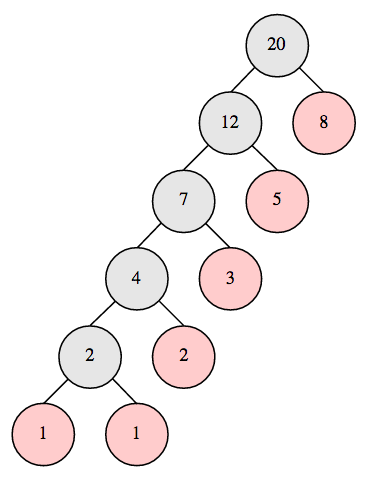
\includegraphics[width=\textwidth*3/10]{huffmanworstcase.png}\\
    \emph{Example of a worst-case height Huffman tree.}
    \end{center}

    In generating the above tree, the internal node generated at the $i$th iteration of the while loop is always used in the $i+1$th iteration, as given by the Fibonacci property  $\sum_{i=1}^n F_i = F_{n+2} - 1$. Therefore, the height of the tree is $m-1$. When generating the encodings, the sum of all the path lengths would be $1 + 2 + 3 + ... (m-1)$. Generating the encodings is thus worst case $O(m^2)$, although this is a \emph{one time operation for a fixed alphabet.}\\

    In the best case, the height of the Huffman tree is given by $\Theta(\log m)$, and we therefore have $\Omega(m \log m)$ as a lower bound for the runtime of generating the encodings table.\\

    \underline{Compression}\\

    Compression of an input string can be performed by iterating through each character and finding the corresponding encoding in the encoding table. This runs in $\Theta(n)$ time, where $n$ is the length of the input.\\

    \end{multicols*}

    \underline{Decompression}\\

    Decompression of an input string can be performed by walking down the Huffman tree for each encoded character and outputting a value whenever a leaf is reached. This also runs in $\Theta(n)$ time, as only one tree edge is traversed for each input character.\\

    An example of building a Huffman tree is shown on the following page.\\

    {\large \underline{LZW Encoding}}\\

    {\large \underline{KMP Substring Search}}\\
    
    {\large \underline{Regular Expressions}}\\

    \newpage

    \begin{center}
    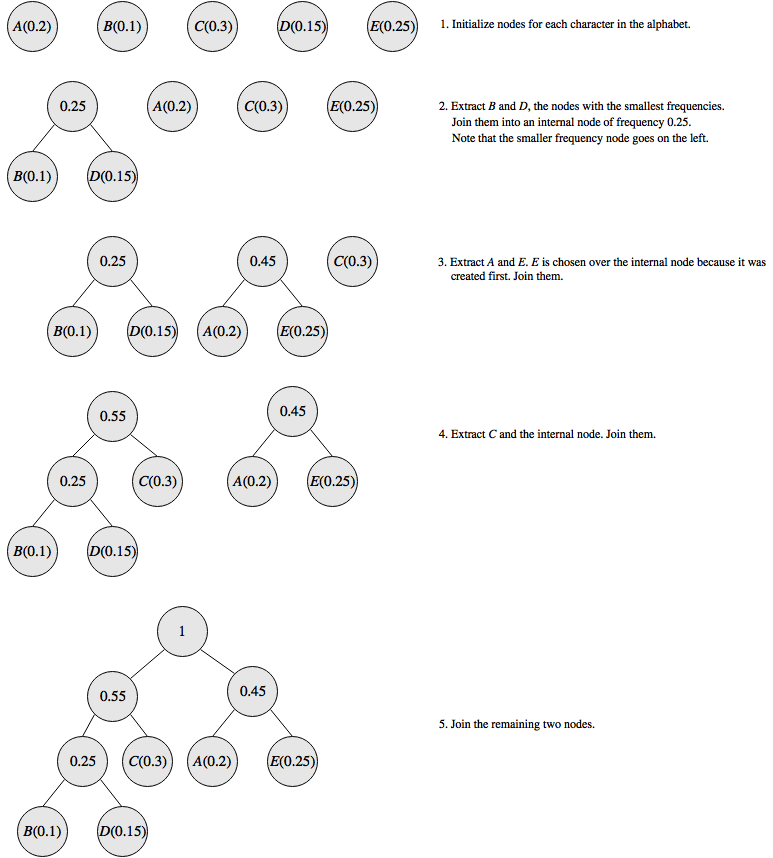
\includegraphics[width=400pt]{huffman.png}\\\vspace{10pt}

    \emph{Example construction of a Huffman tree given the alphabet $\{A:0.2, B:0.1, C:0.3, D:0.15, E:0.25\}$.}\\\vspace{10pt}

    \begin{tabular}{|c|l|}\hline
        \textbf{A}&$10$\\\hline
        \textbf{B}&$000$\\\hline
        \textbf{C}&$01$\\\hline
        \textbf{D}&$001$\\\hline
        \textbf{E}&$11$\\\hline
    \end{tabular}\\\vspace{10pt}

    \emph{Encoding table.}
    \end{center}

    \newpage

    \begin{multicols*}{2}

\end{multicols*}

\end{document}
